\documentclass[12pt]{article}
\usepackage[utf8]{inputenc}
\usepackage[spanish]{babel}
\usepackage{geometry}
\usepackage{titlesec}
\usepackage{url}
\usepackage{amsmath}
\usepackage{graphicx}
\usepackage{lmodern}
\usepackage{hyperref}

\geometry{margin=2.5cm}

\titleformat{\section}{\large\bfseries}{\thesection}{1em}{}

\title{Validación del lado del cliente vs. del lado del servidor}
\date{}

\begin{document}

\maketitle

\section*{Validación del lado del cliente vs. del lado del servidor}

La validación de entrada debe implementarse en el servidor antes de que las funciones de una aplicación procesen los datos, ya que cualquier validación de entrada basada en JavaScript realizada en el cliente puede ser eludida por un atacante que deshabilite JavaScript o utilice un proxy web.

Se recomienda implementar tanto la validación basada en JavaScript del lado del cliente para la experiencia de usuario (UX), como la validación del lado del servidor para garantizar la seguridad, aprovechando cada una por sus respectivas ventajas.

\subsection*{Lado del servidor}
- Protege la lógica del sistema. \\
- No puede ser eludido por el usuario final. \\
- Es esencial para la integridad y seguridad de la aplicación.

\begin{figure}[h!]
  \centering
  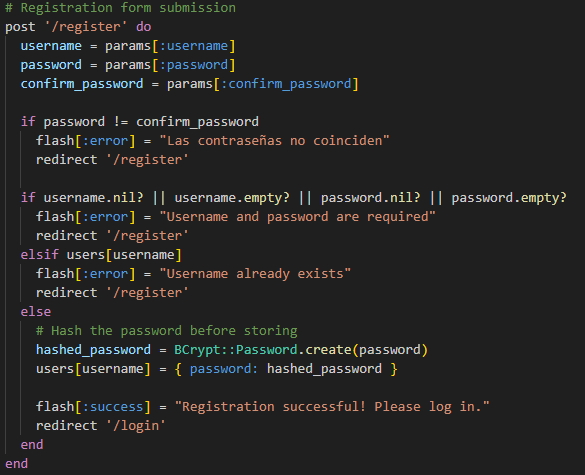
\includegraphics[width=0.6\textwidth]{first.png}
  \caption{Porcion de codigo tomado desde la parte del servidor.}
  \label{fig:ejemplo}
\end{figure}

\subsection*{Lado del cliente}
- Mejora la experiencia del usuario (UX). \\
- Permite respuestas más rápidas sin necesidad de esperar una respuesta del servidor. \\
- Puede ser manipulado o deshabilitado por usuarios maliciosos.
\begin{figure}[h!]
  \centering
  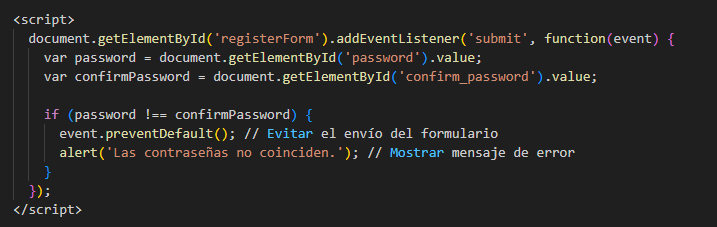
\includegraphics[width=0.6\textwidth]{second.png}
  \caption{Porcion de codigo tomado desde la parte del cliente.}
  \label{fig:ejemplo}
\end{figure}
\footnote{Fuente: OWASP, https://cheatsheetseries.owasp.org/cheatsheets/Input_Validation_Cheat_Sheet.html}.

\end{document}
